\documentclass[a4paper,12pt]{article}
\usepackage{amsmath}
\usepackage{graphicx}
\usepackage{booktabs}
\usepackage{geometry}
\geometry{margin=1in}
\usepackage{float}

\title{\textbf{Lab Report: Custom Weighted Summing \& Difference Amplifier, Op-Amp Integrator, and Precision Rectifier}}
\author{EE24BTECH11048-NITHIN.K\\EE24BTECH11021-ESHAN RAY}
\date{\today}

\begin{document}

\maketitle

\section{Objective}
The purpose of this experiment is to design and implement a custom weighted summing and difference amplifier circuit using an operational amplifier, to study the working of an op-amp integrator, and to analyze the behavior of a precision rectifier (super diode). The circuits perform the following mathematical functions:
\begin{equation}
    V_{out} = 2V_1 + V_2 - V_3
\end{equation}
\begin{equation}
    V_{out} = 2V_1 - V_3
\end{equation}
\begin{equation}
    V_{out} = - \frac{1}{RC} \int V_{in} dt
\end{equation}
\begin{equation}
    V_{out} = \begin{cases} 
        0, & V_{in} < 0 \\ 
        V_{in}, & V_{in} > 0
    \end{cases}
\end{equation}
\section{Components Required}
\begin{itemize}
    \item Operational amplifier (LM741, TL081, LM358, or equivalent)
    \item Resistors (values chosen to achieve desired functionality)
    \item Capacitor (for integration circuit)
    \item Diode (e.g., 1N4148 for precision rectifier)
    \item DC power supply (\( \pm 15V \))
    \item Function generator (to provide input signals)
    \item Oscilloscope (to observe output waveforms)
\end{itemize}

\section{Circuit Design}
\subsection{Summing and Difference Amplifier}
To implement the given equations, the following resistor values are selected:

For \( V_{out} = 2V_1 + V_2 - V_3 \):
\begin{itemize}
    \item \( R_1 = R_3 = 10k\Omega \)
    \item \( R_2 = 20k\Omega \)
    \item \( R_f = 20k\Omega \)
\end{itemize}

For \( V_{out} = 2V_1 - V_3 \):
\begin{itemize}
    \item \( R_1 = 10k\Omega \)
    \item \( R_3 = 10k\Omega \)
    \item \( R_f = 20k\Omega \)
    \item No \( R_2 \) needed (open circuit)
\end{itemize}

\subsection{Op-Amp Integrator}
For the integrator circuit, the component values are chosen as follows:
\begin{itemize}
    \item \( R = 10k\Omega \)
    \item \( C = 0.1\mu F \)
\end{itemize}

\subsection{Precision Rectifier}
For the precision rectifier:
\begin{itemize}
    \item Op-amp (LM358 or TL081)
    \item Diode (1N4148)
    \item Resistors (as per design)
\end{itemize}

\section{Experimental Procedure}
\begin{enumerate}
    \item Assemble the circuits on a breadboard as per the schematic.
    \item Apply \( \pm 15V \) DC power to the op-amp.
    \item Use the function generator to apply the appropriate input signals.
    \item Observe and record the output waveforms using an oscilloscope.
    \item Compare the measured output with the theoretically expected values.
\end{enumerate}


\section{Theory and Comparison in Observations}
\begin{table}[H]
    \centering
    \begin{tabular}{|c|c|c|}
        \hline
        \textbf{Input Signals} & \textbf{Expected \( V_{out} \)} & \textbf{Measured \( V_{out} \)} \\
        \hline
        \( V_1 = 5V, V_2 = 3V, V_3 = 3V \) & \( 2(5) + 3 - 3 = 10V \) & \( 9.201V \) \\
        \hline
        \( V_1 = 5V, V_3 = 3V \) & \( 2(5) - 3 = 7V \) & \( 7.V \) \\
        \hline
        Square wave input (Integrator) & Triangular wave output & Observed triangular wave \\
        \hline
        Small AC signal (Rectifier) & Positive half-cycle only & Observed rectified waveform \\
        \hline
    \end{tabular}
    \caption{Experimental Results}
    \label{tab:results}
\end{table}

Operational amplifiers (op-amps) can be used to perform mathematical operations such as addition, subtraction, scaling, integration, and precision rectification.

\subsection{Summing and Difference Amplifier}
The inverting summing amplifier is used to achieve the desired weighted sum of input voltages. The general equation for an inverting summing amplifier is:
\begin{equation}
    V_{out} = -\left( \frac{R_f}{R_1} V_1 + \frac{R_f}{R_2} V_2 + \frac{R_f}{R_3} V_3 \right)
\end{equation}
By carefully selecting resistor values, the required coefficients in the equation can be achieved. If a non-inverting input is required, a combination of inverting and summing amplifiers can be used.
\begin{figure}[H]
    \centering
    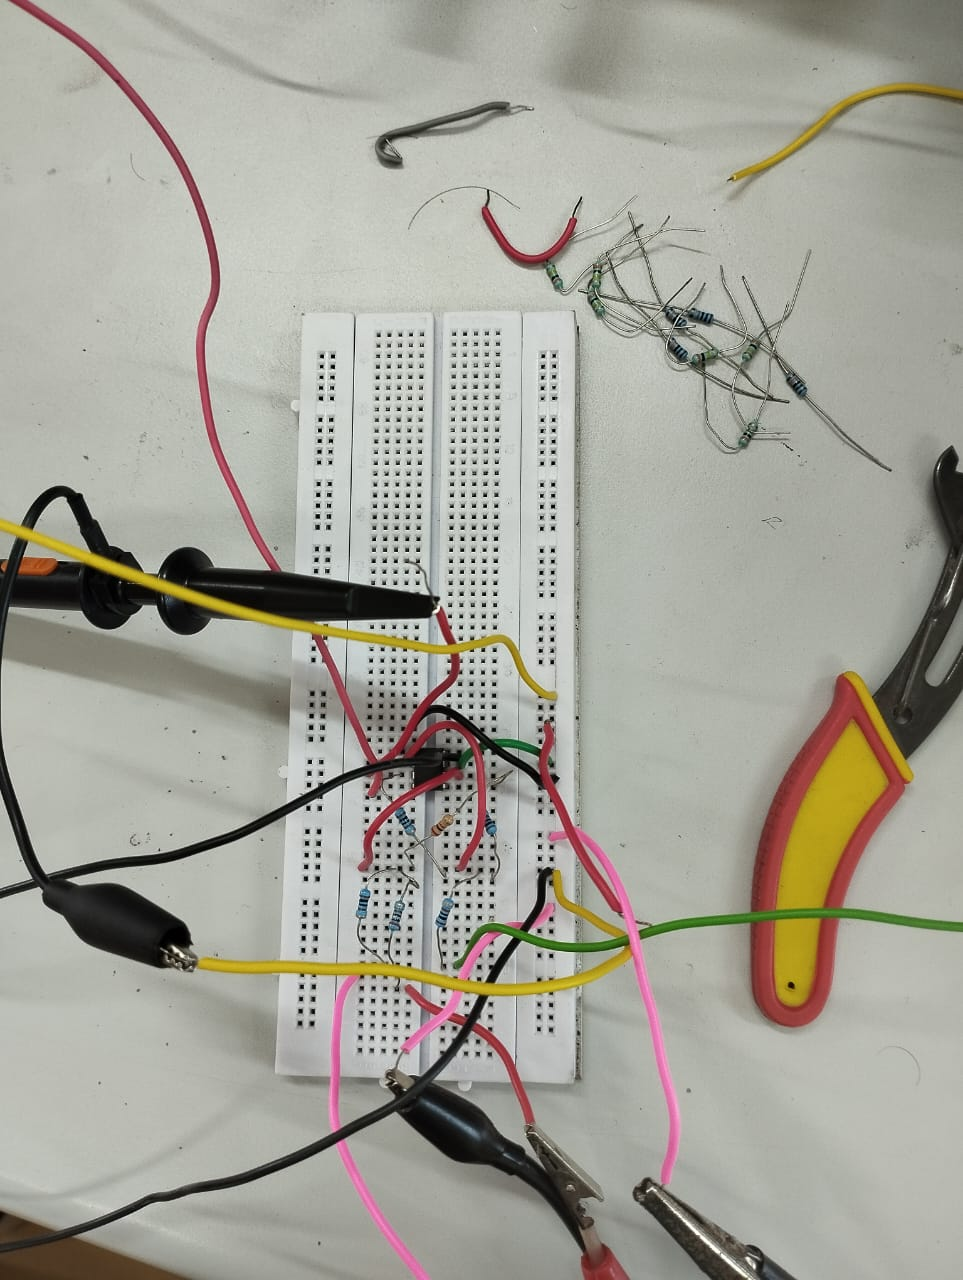
\includegraphics[width=0.4\textwidth]{figs/addercircuit.png}
    \caption{Circuit Diagram In Experiment}
\end{figure}
\begin{figure}[H]
    \centering
    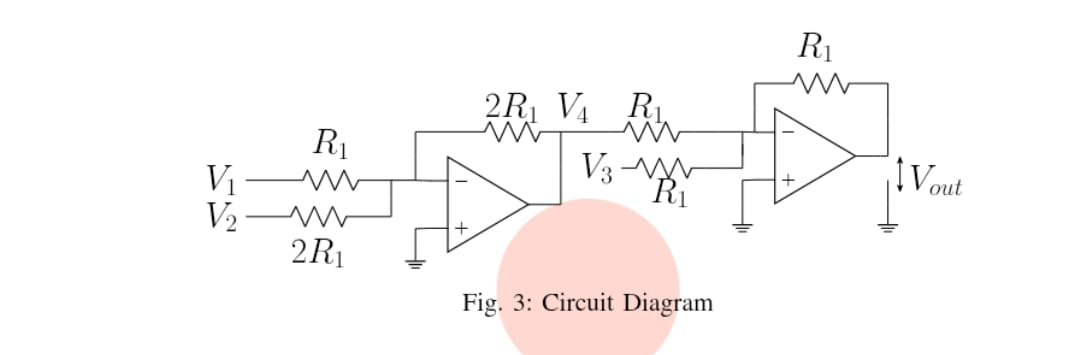
\includegraphics[width=0.5\textwidth]{figs/adder_ideal.png}
    \caption{Circuit Diagram}
\end{figure}
\begin{figure}[H]
    \centering
    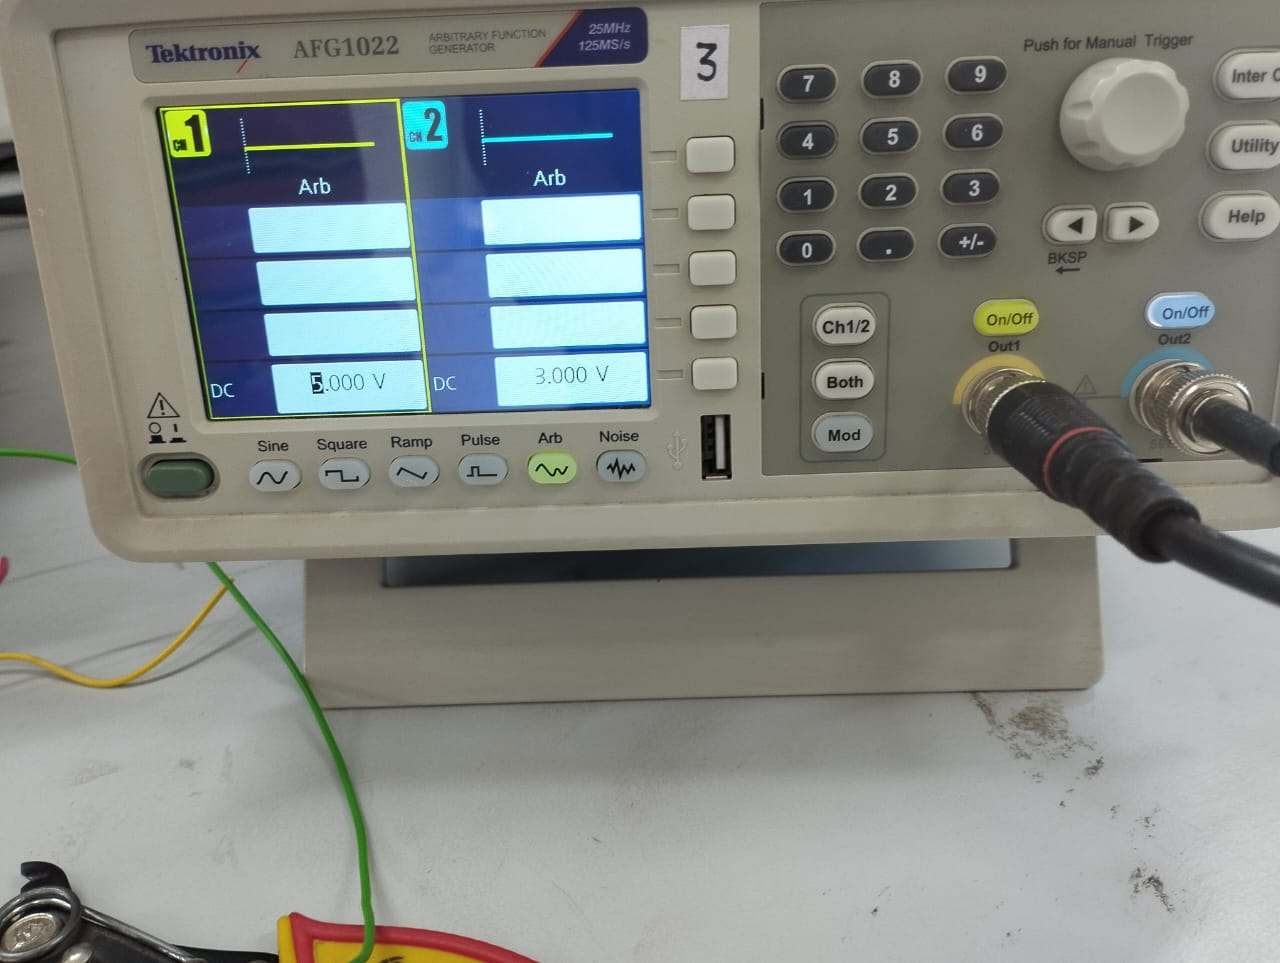
\includegraphics[width=0.5\textwidth]{figs/adderv1v2.png}
    \caption{Voltage $V_1 = 5V$ and $V_2 = 3V$ for $2V_1 + V_2 - V_3$}
\end{figure}
\begin{figure}[H]
    \centering
    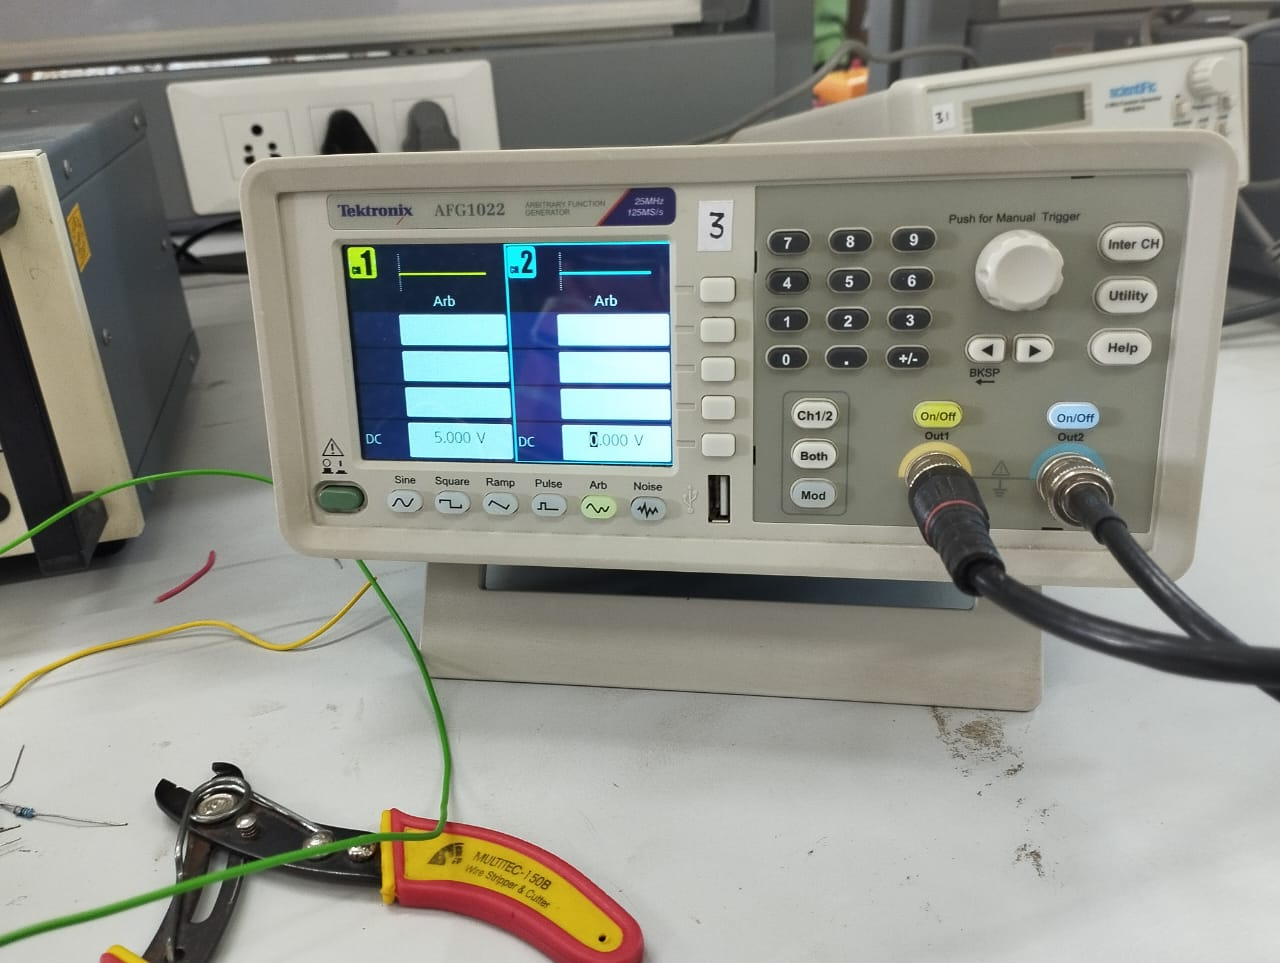
\includegraphics[width=0.5\textwidth]{figs/adderv1.png}
    \caption{Voltage $V_1 = 5V$ and $V_2 = 0V$ for $2V_1 - V_3$}
\end{figure}
\begin{figure}[H]
    \centering
    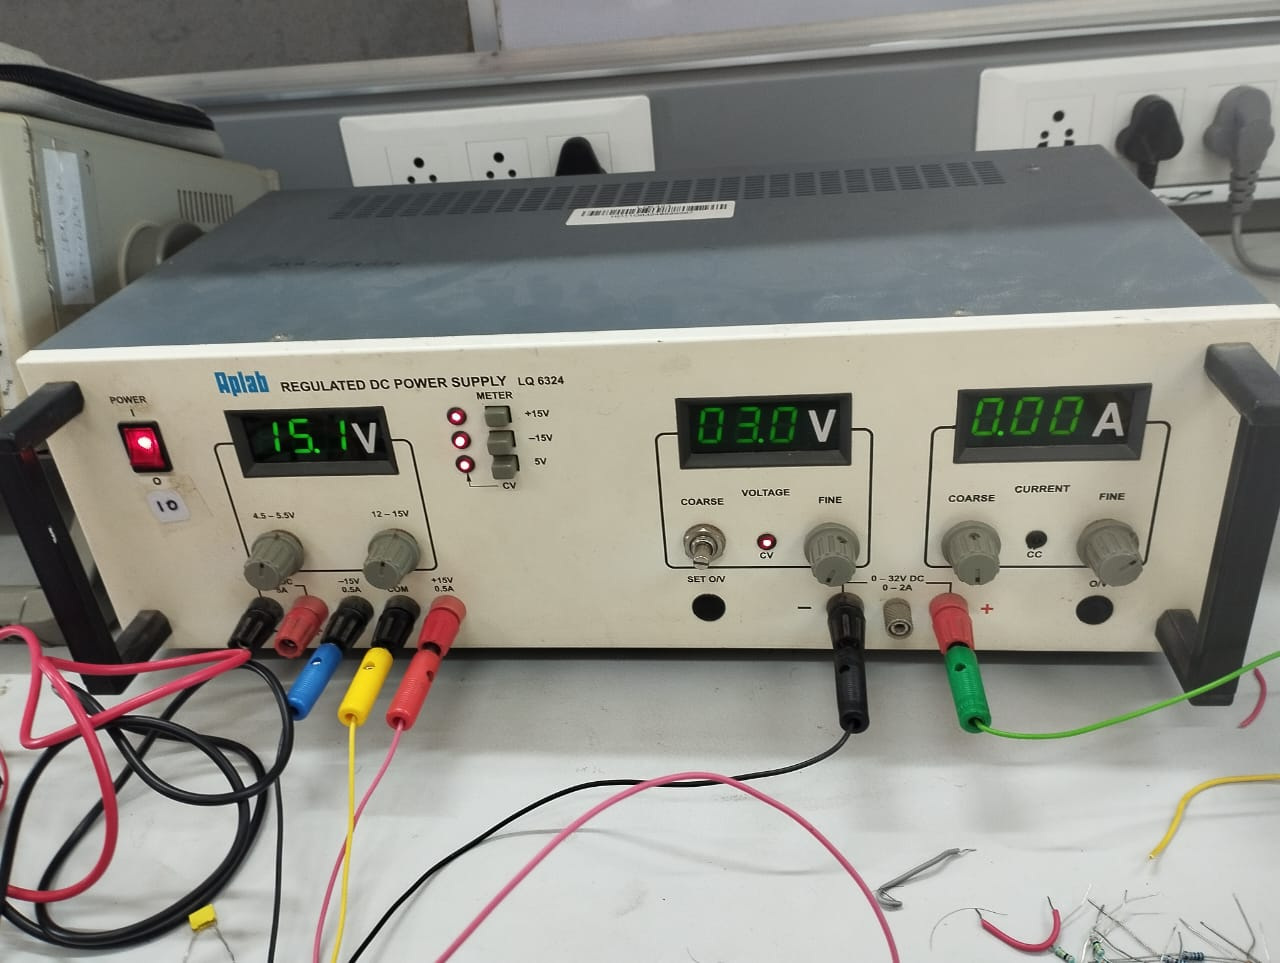
\includegraphics[width=0.5\textwidth]{figs/adderv3.png}
    \caption{Voltage $V_3 = 3V$}
\end{figure}

\begin{figure}[H]
    \centering
    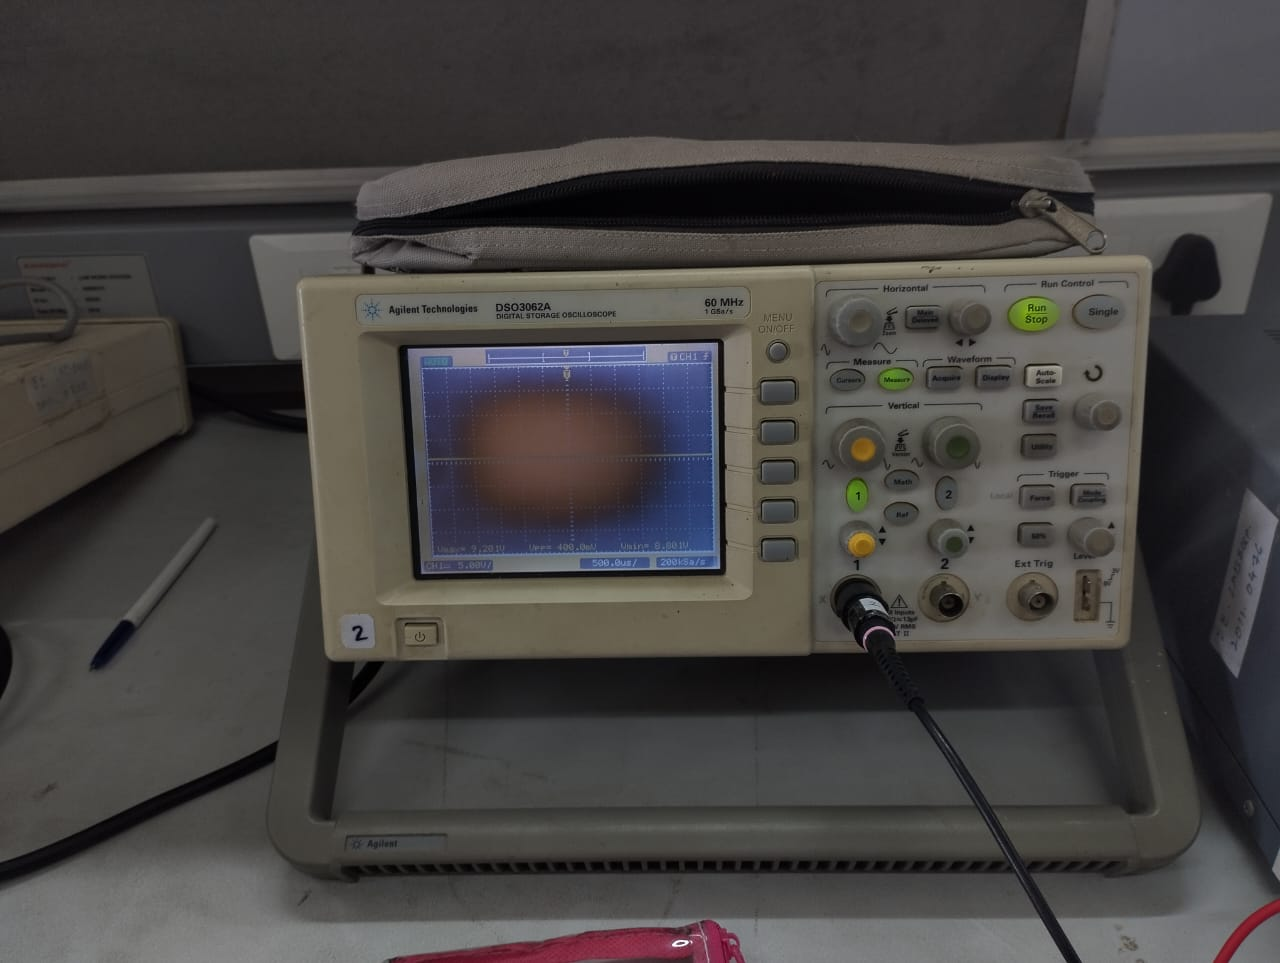
\includegraphics[width=0.5\textwidth]{figs/addervalue2.png}
    \caption{Observed value for $2V_1 + V_2 - V_3$}
\end{figure}
\begin{figure}[H]
    \centering
    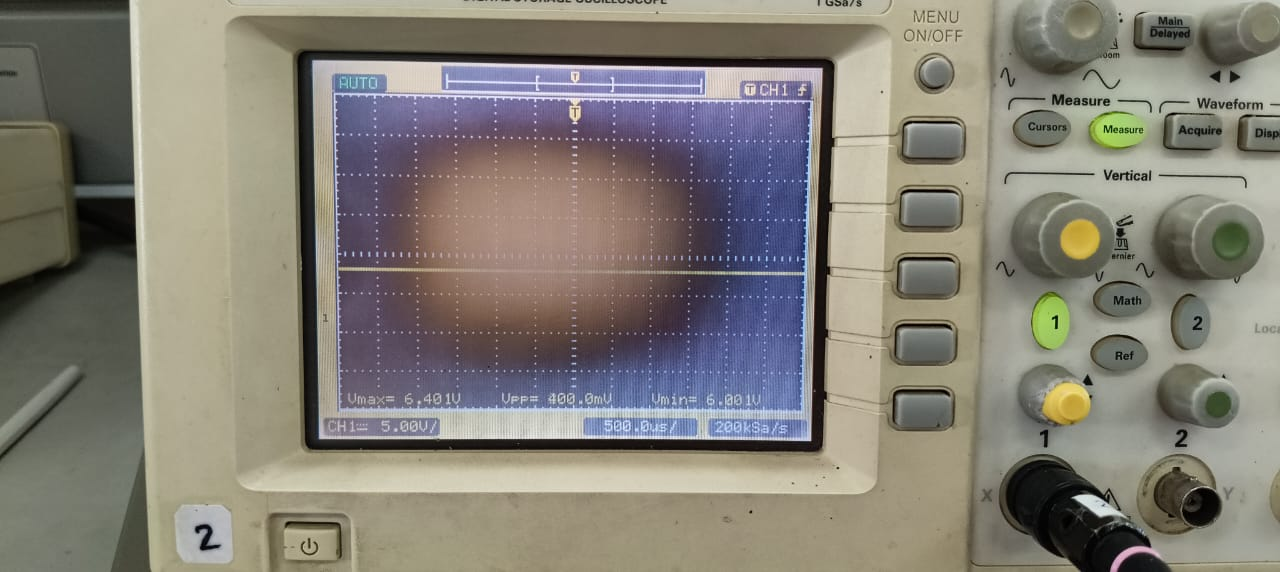
\includegraphics[width=0.5\textwidth]{figs/addervalue1.png}
    \caption{Observed value for $2V_1 - V_3$}
\end{figure}
\subsection{Op-Amp Integrator}
The op-amp integrator performs the mathematical integration of an input signal. It consists of an operational amplifier with a capacitor in the feedback path instead of a resistor. The integrator follows the equation:
\begin{equation}
    V_{out} = - \frac{1}{RC} \int V_{in} dt
\end{equation}
This circuit converts a square wave input into a triangular wave output and is widely used in signal processing applications.
\begin{figure}[H]
    \centering
    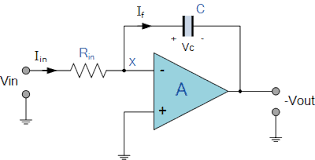
\includegraphics[width=0.6\textwidth]{figs/integratorcircuit.png}
    \caption{Circuit Diagram}
\end{figure}
\begin{figure}[H]
    \centering
    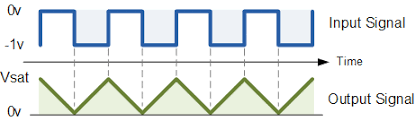
\includegraphics[width=0.7\textwidth]{figs/integrator_ideal.png}
    \caption{Input and Output Signal for Integrator}
\end{figure}
\begin{figure}[H]
    \centering
    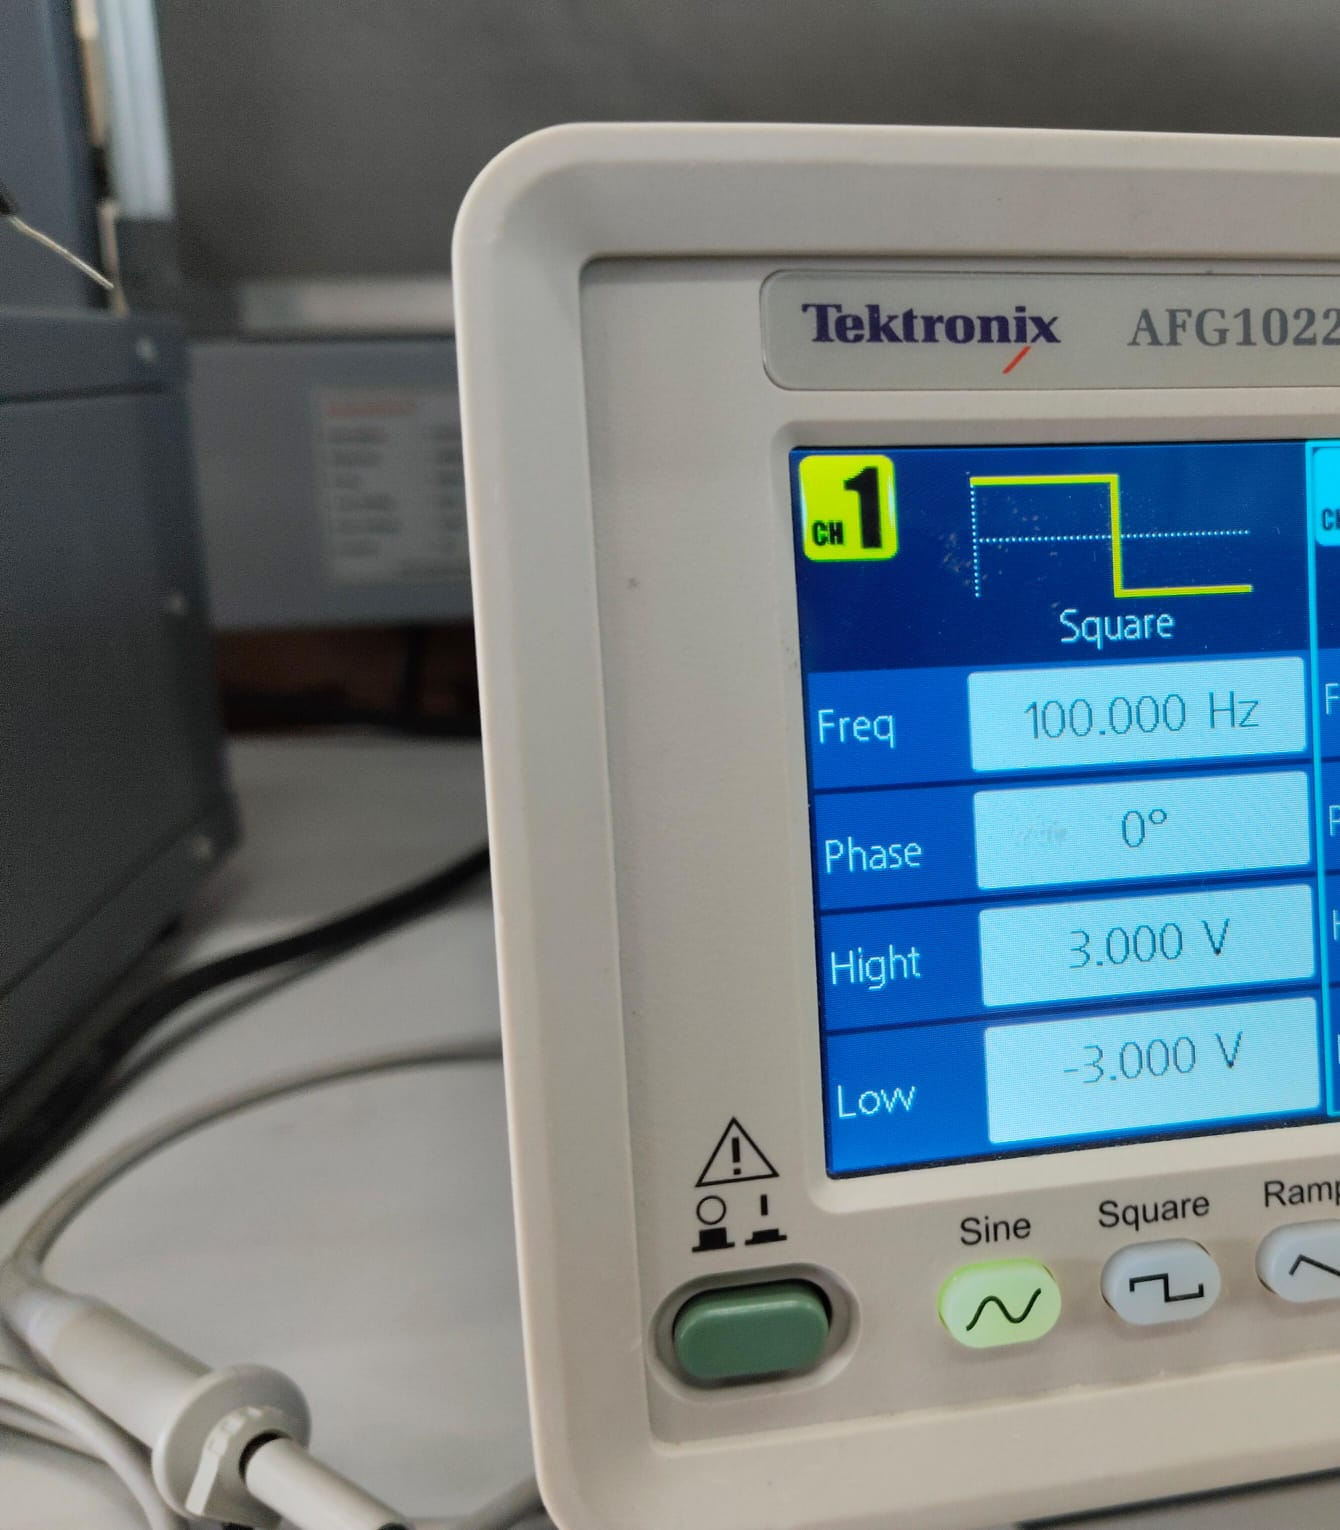
\includegraphics[width=0.5\textwidth]{figs/integrator2.png}
    \caption{Input Signal In function generator}
\end{figure}
\begin{figure}[H]
    \centering
    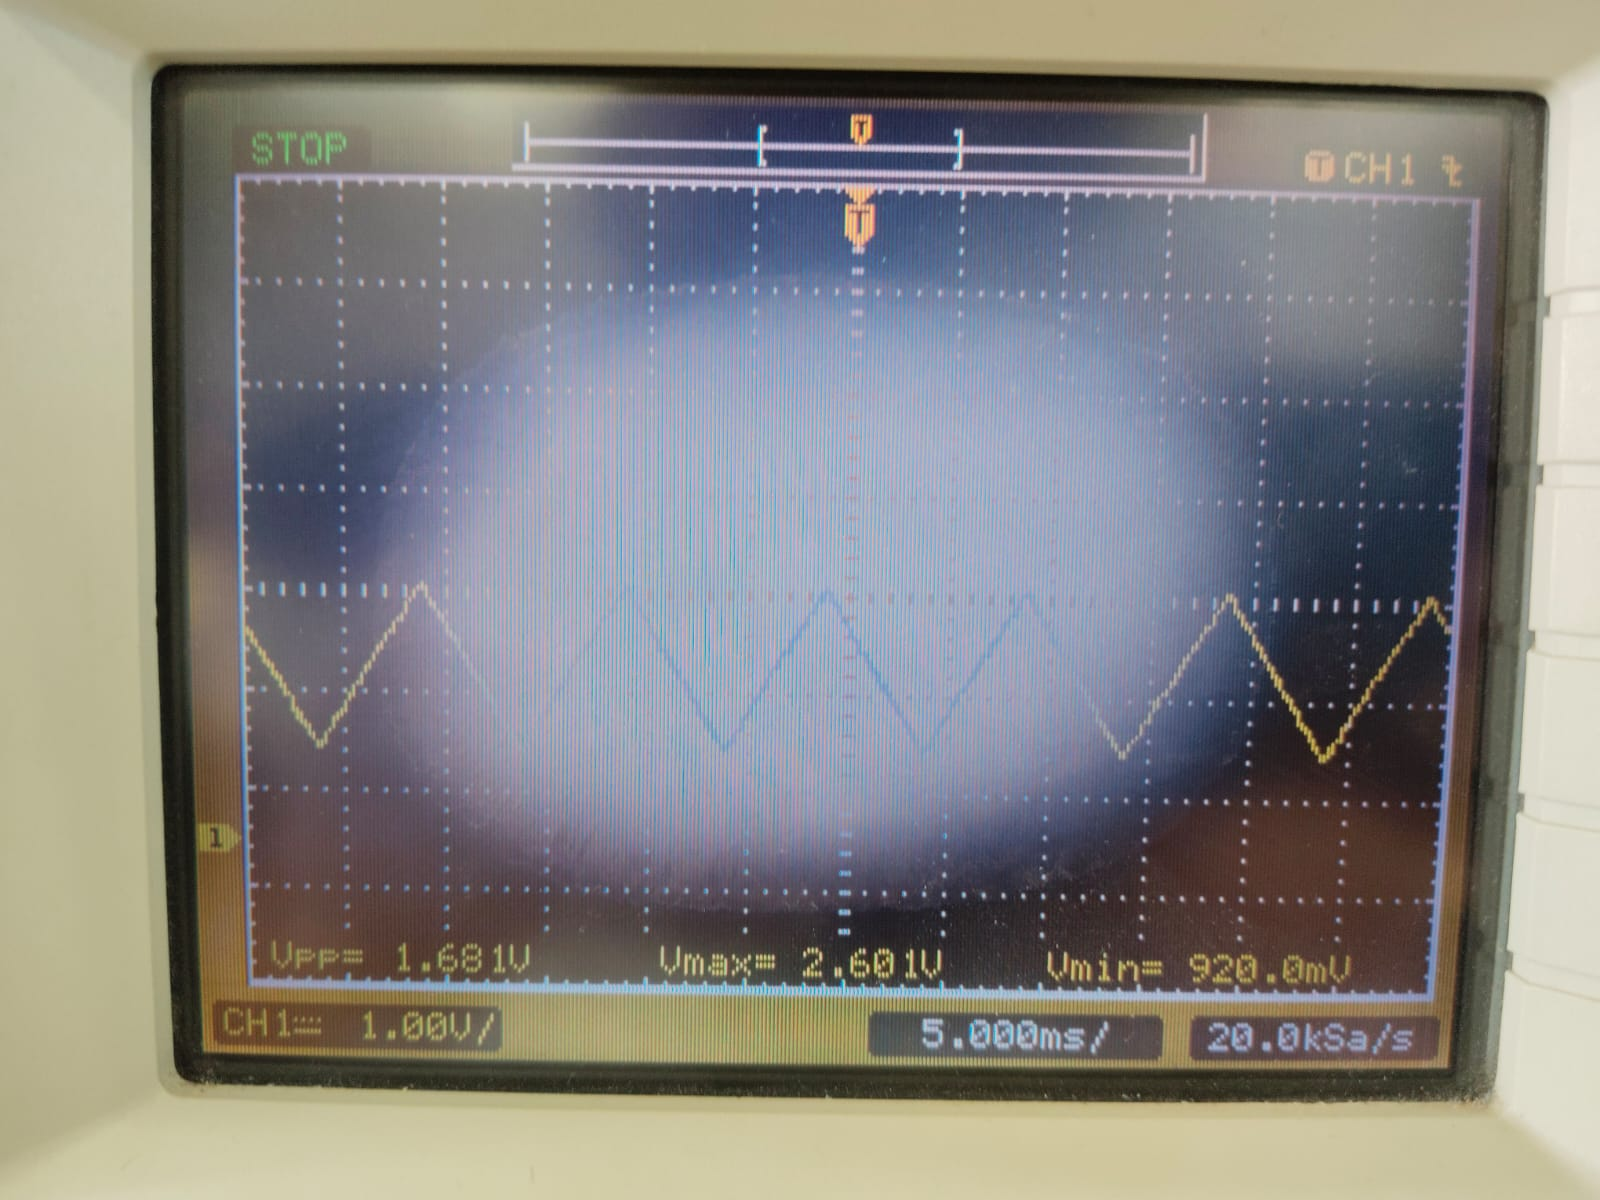
\includegraphics[width=0.5\textwidth]{figs/integrator1.png}
    \caption{Observed Output Signal}
\end{figure}
The peak output voltage of an op-amp integrator with a square wave input is:

\[
V_{\text{out max}} = \frac{V_{\text{in max}}}{RC} \times \frac{1}{2f}
\]

Given:
\[
V_{\text{in max}} = 3V, \quad R = 10k\Omega, \quad C = 0.1\mu F, \quad f = 1kHz
\]

Substituting the values:

\[
V_{\text{out max}} = \frac{3}{(10k\Omega \times 0.1\mu F)} \times \frac{1}{2 \times 1000}
\]

\[
= \frac{3}{(10^4 \times 10^{-7})} \times \frac{1}{2000}
\]

\[
= \frac{3}{10^{-3}} \times \frac{1}{2000}
\]

\[
= 3000 \times \frac{1}{2000}
\]

\[
= 1.5V
\]

Thus, the peak output voltage is:

\[
V_{\text{out max}} = 1.5V
\]
The observed peak output is $2.6V - 0.92V = 1.68V$.
\subsection{Precision Rectifier (Super Diode)}
A precision rectifier, or super diode, eliminates the voltage drop problem of conventional diodes, enabling rectification of small AC signals. The circuit consists of an op-amp controlling a diode. For a half-wave rectifier:
\begin{equation}
    V_{out} = \begin{cases} 
        0, & V_{in} < 0 \\ 
        V_{in}, & V_{in} > 0
    \end{cases}
\end{equation}
A full-wave rectifier can be implemented using an additional summing stage to combine the positive and inverted negative portions.

\begin{figure}[H]
    \centering
    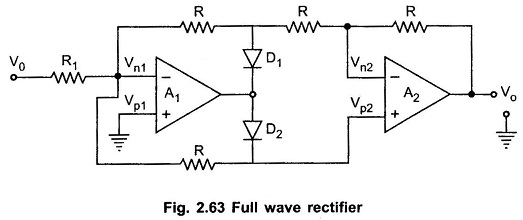
\includegraphics[width=0.5\textwidth]{figs/fullwave_ideal.png}
    \caption{Circuit Diagram for halfwave}
\end{figure}
\begin{figure}[H]
    \centering
    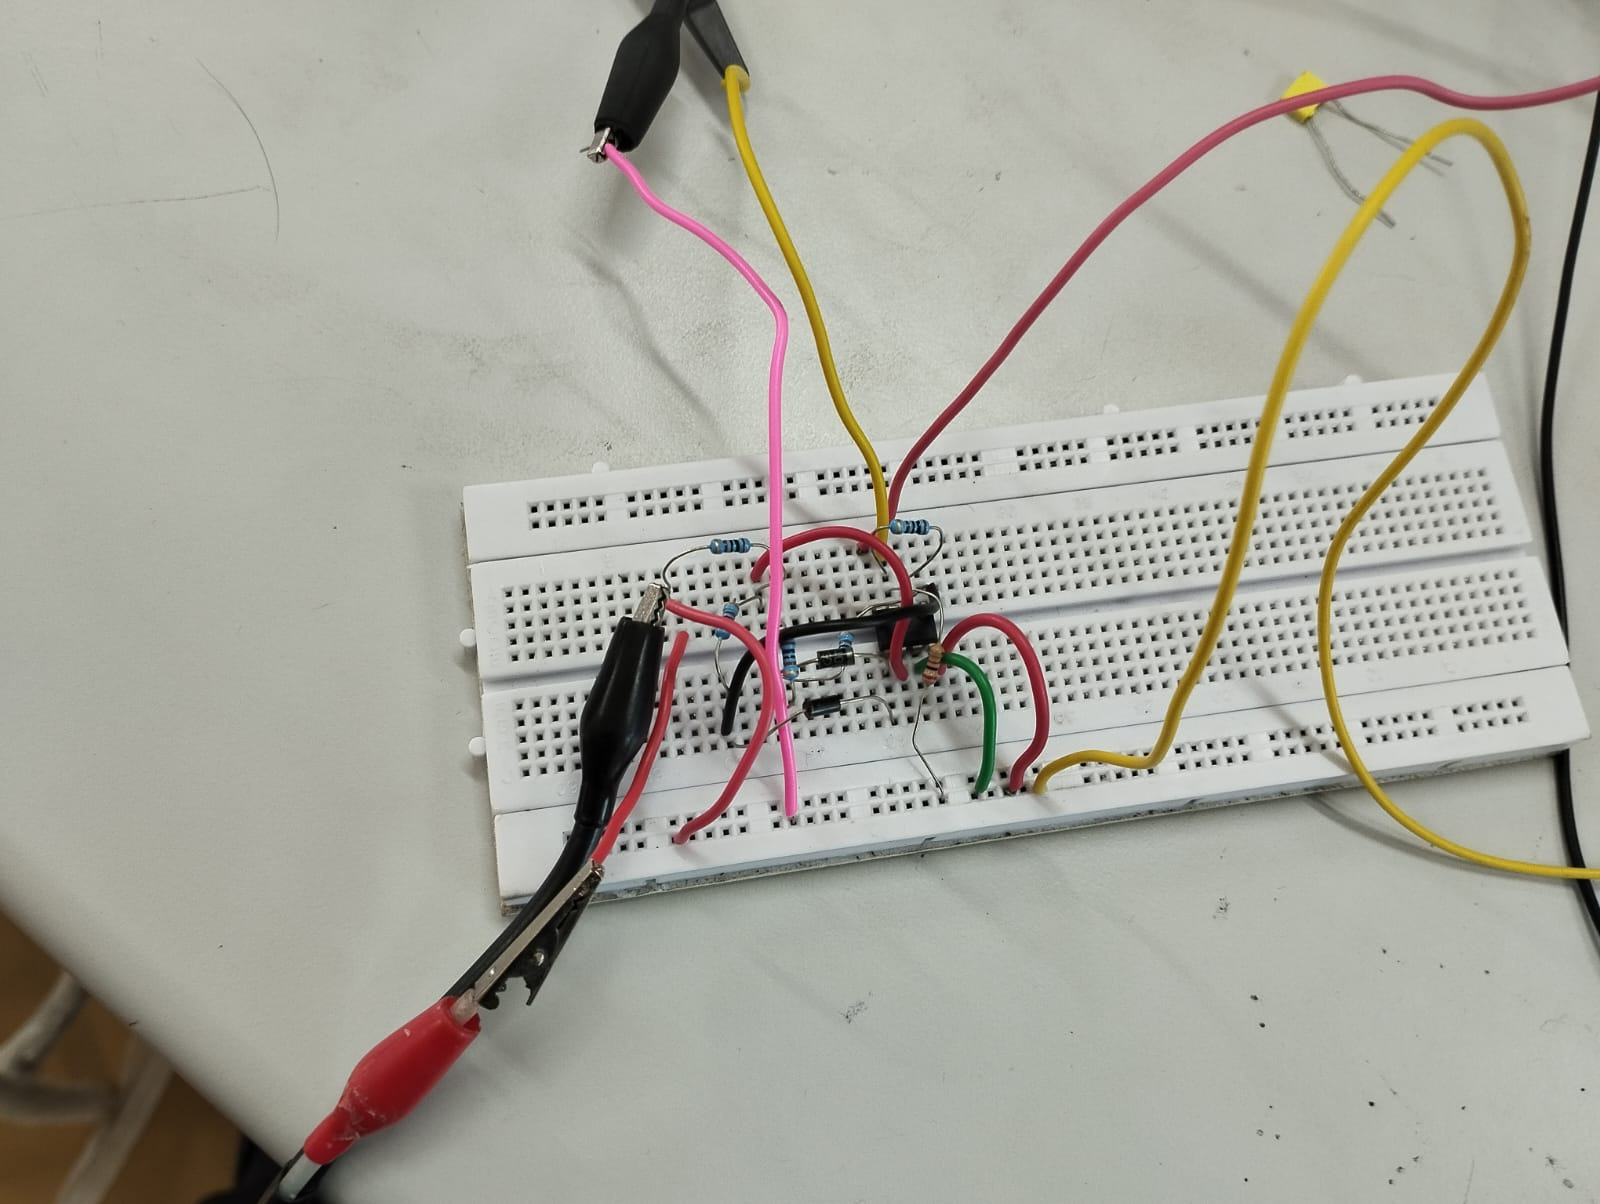
\includegraphics[width=0.5\textwidth]{figs/fullwave2.png}
    \caption{Circuit Diagram In Experiment for fullwave}
\end{figure}
\begin{figure}[H]
    \centering
    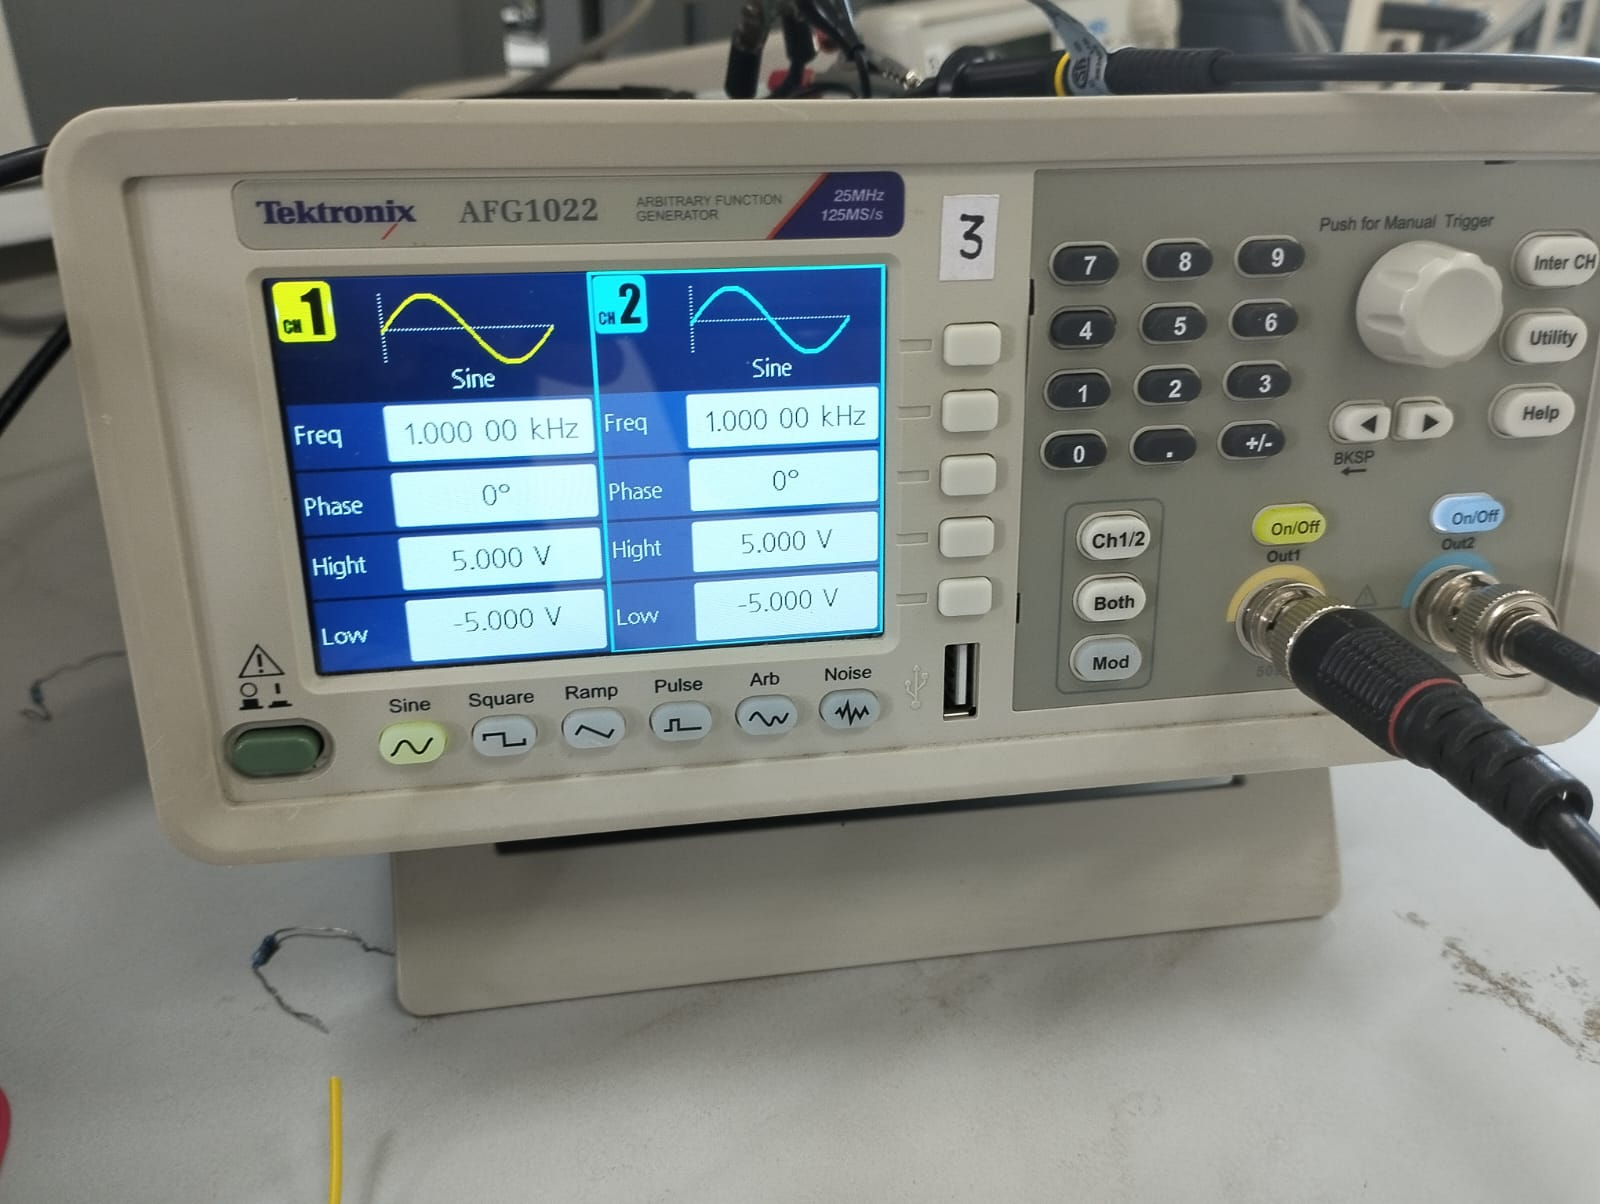
\includegraphics[width=0.5\textwidth]{figs/fullwave3.png}
    \caption{Input Values given by function generator for fullwave}
\end{figure}
\begin{figure}[H]
    \centering
    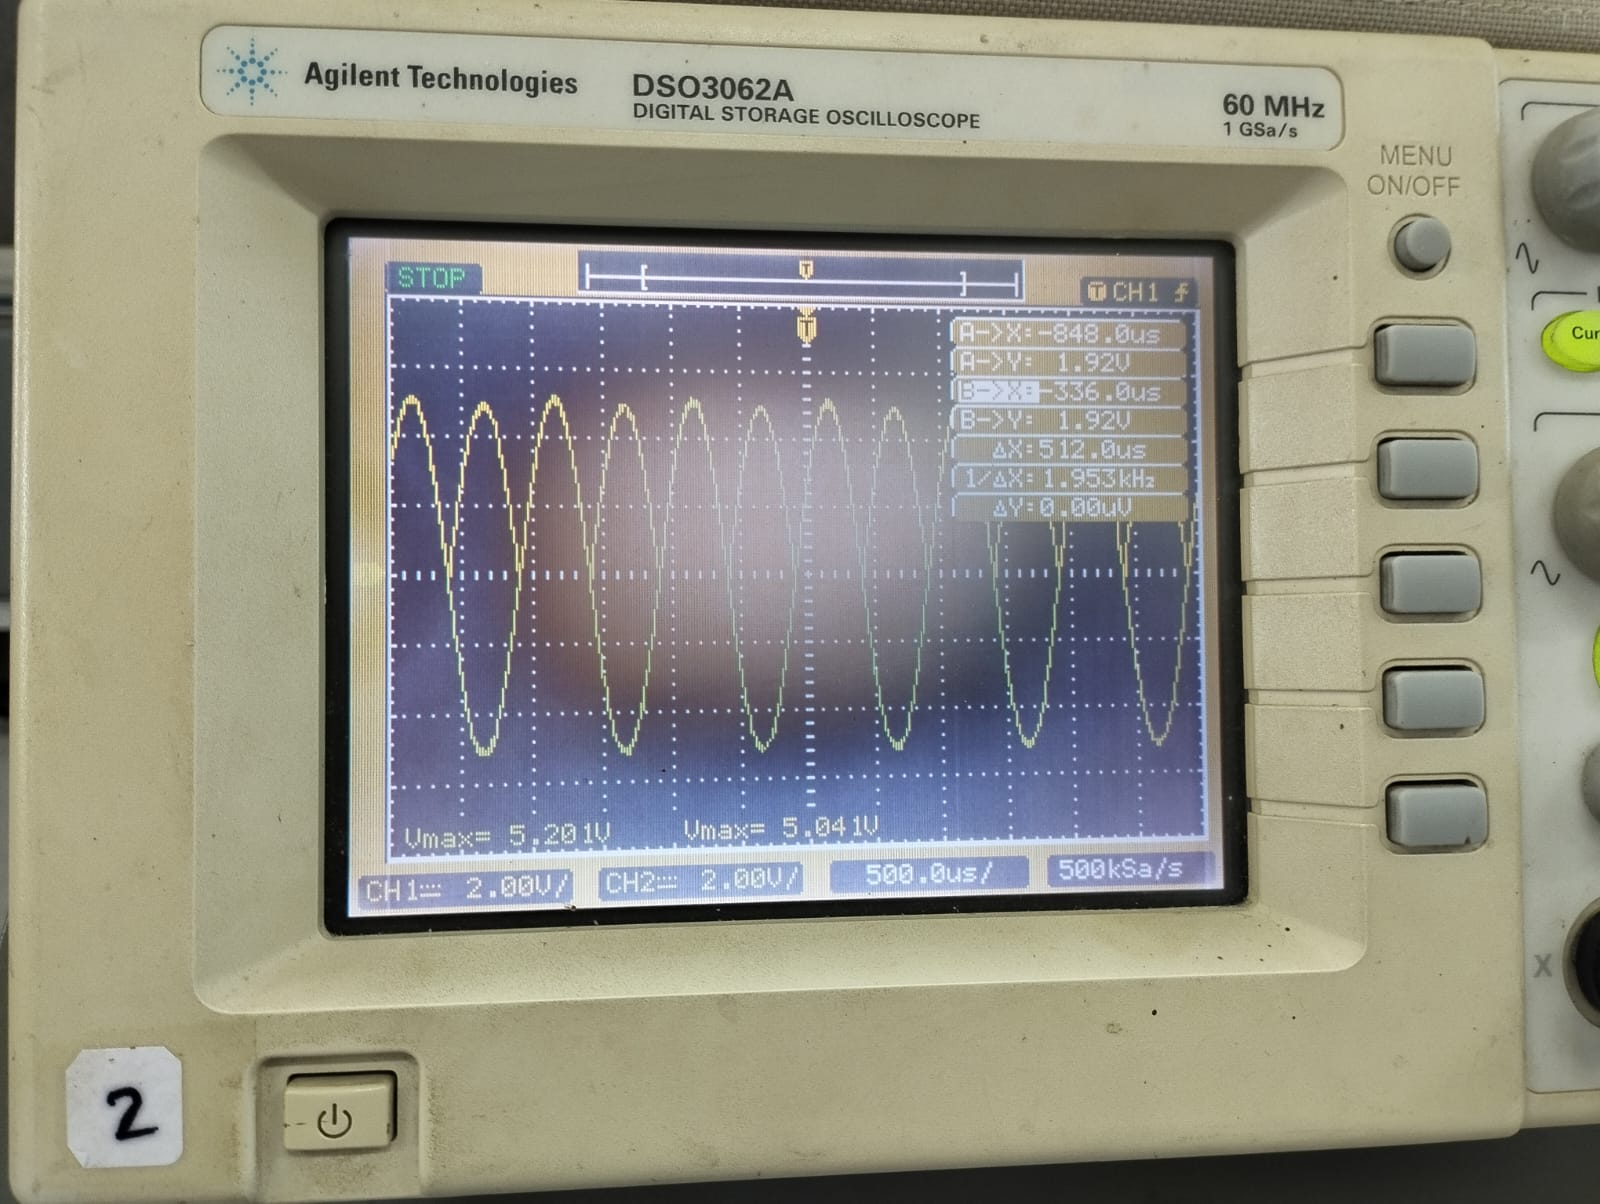
\includegraphics[width=0.5\textwidth]{figs/fullwave1.png}
    \caption{Observed Fullwave Rectification}
\end{figure}
\begin{figure}[H]
    \centering
    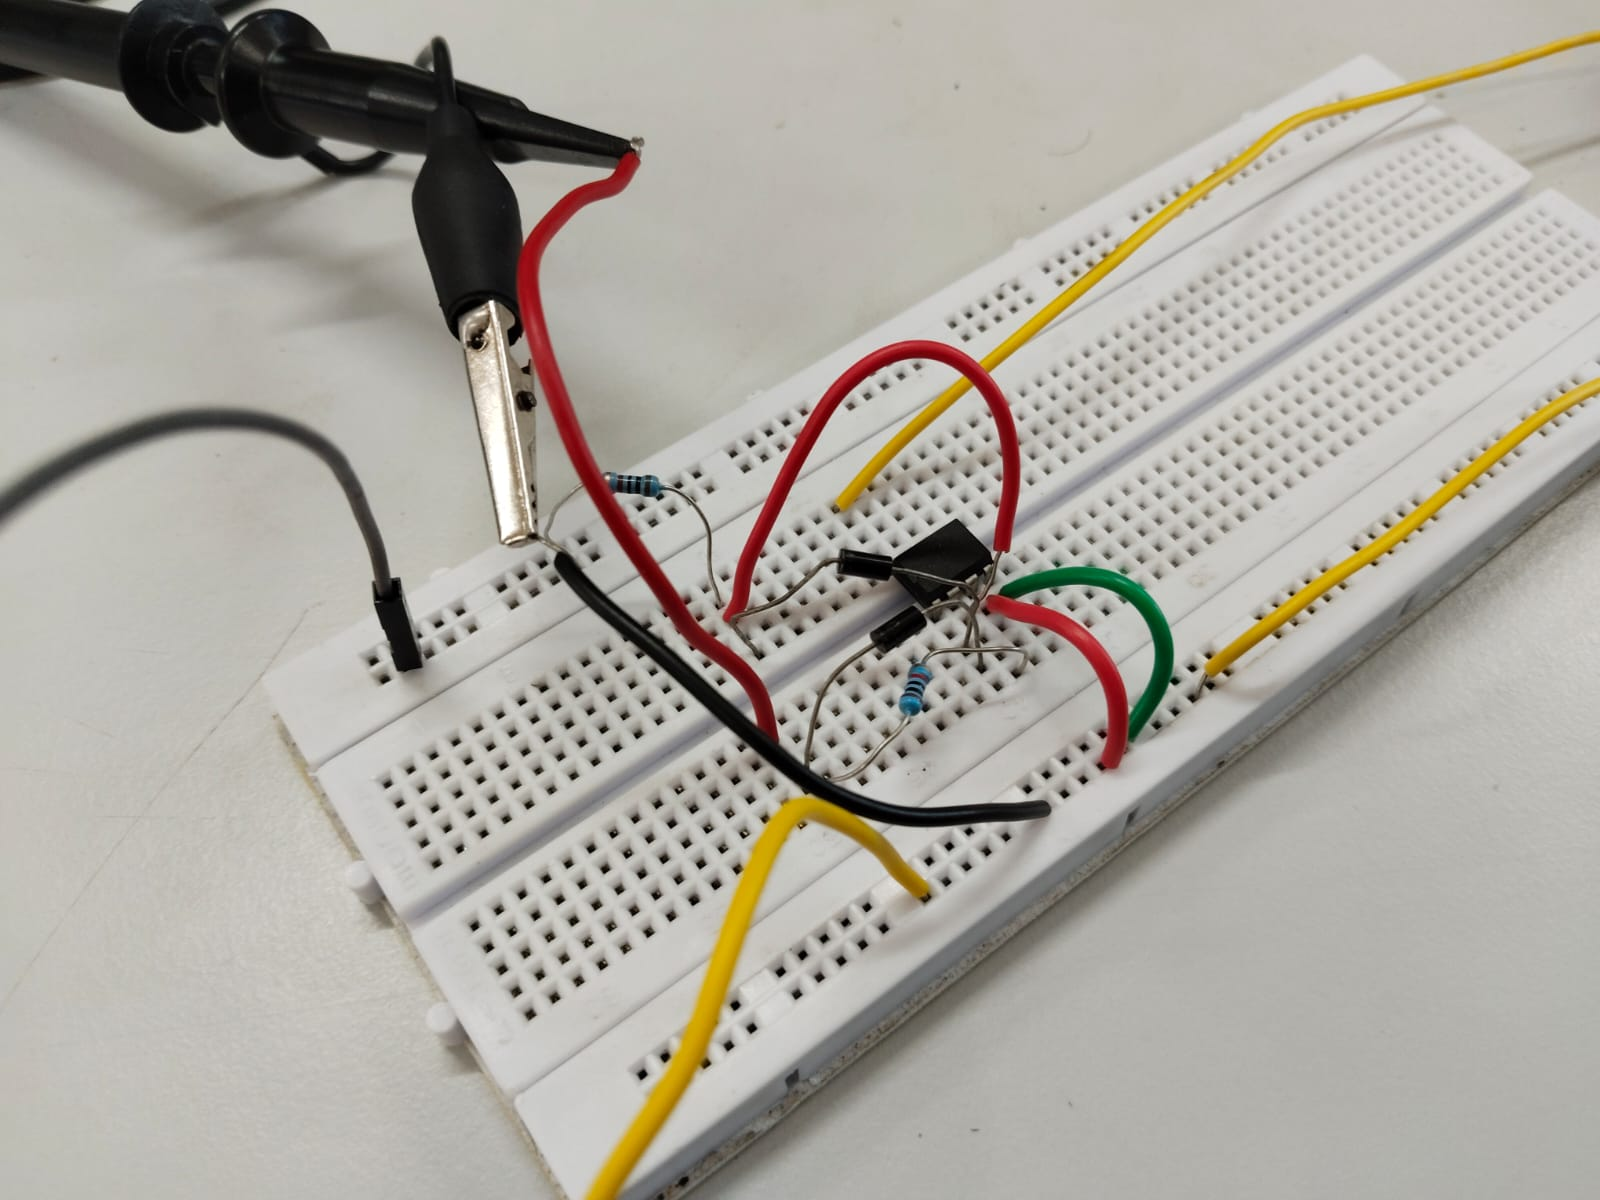
\includegraphics[width=0.5\textwidth]{figs/halfwavecircuit.png}
    \caption{Circuit Diagram In Experiment for halfwave}
\end{figure}
\begin{figure}[H]
    \centering
    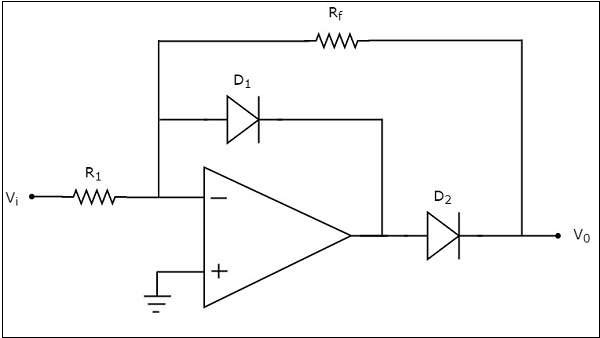
\includegraphics[width=0.5\textwidth]{figs/halfwave_ideal.png}
    \caption{Circuit Diagram for halfwave}
\end{figure}
\begin{figure}[H]
    \centering
    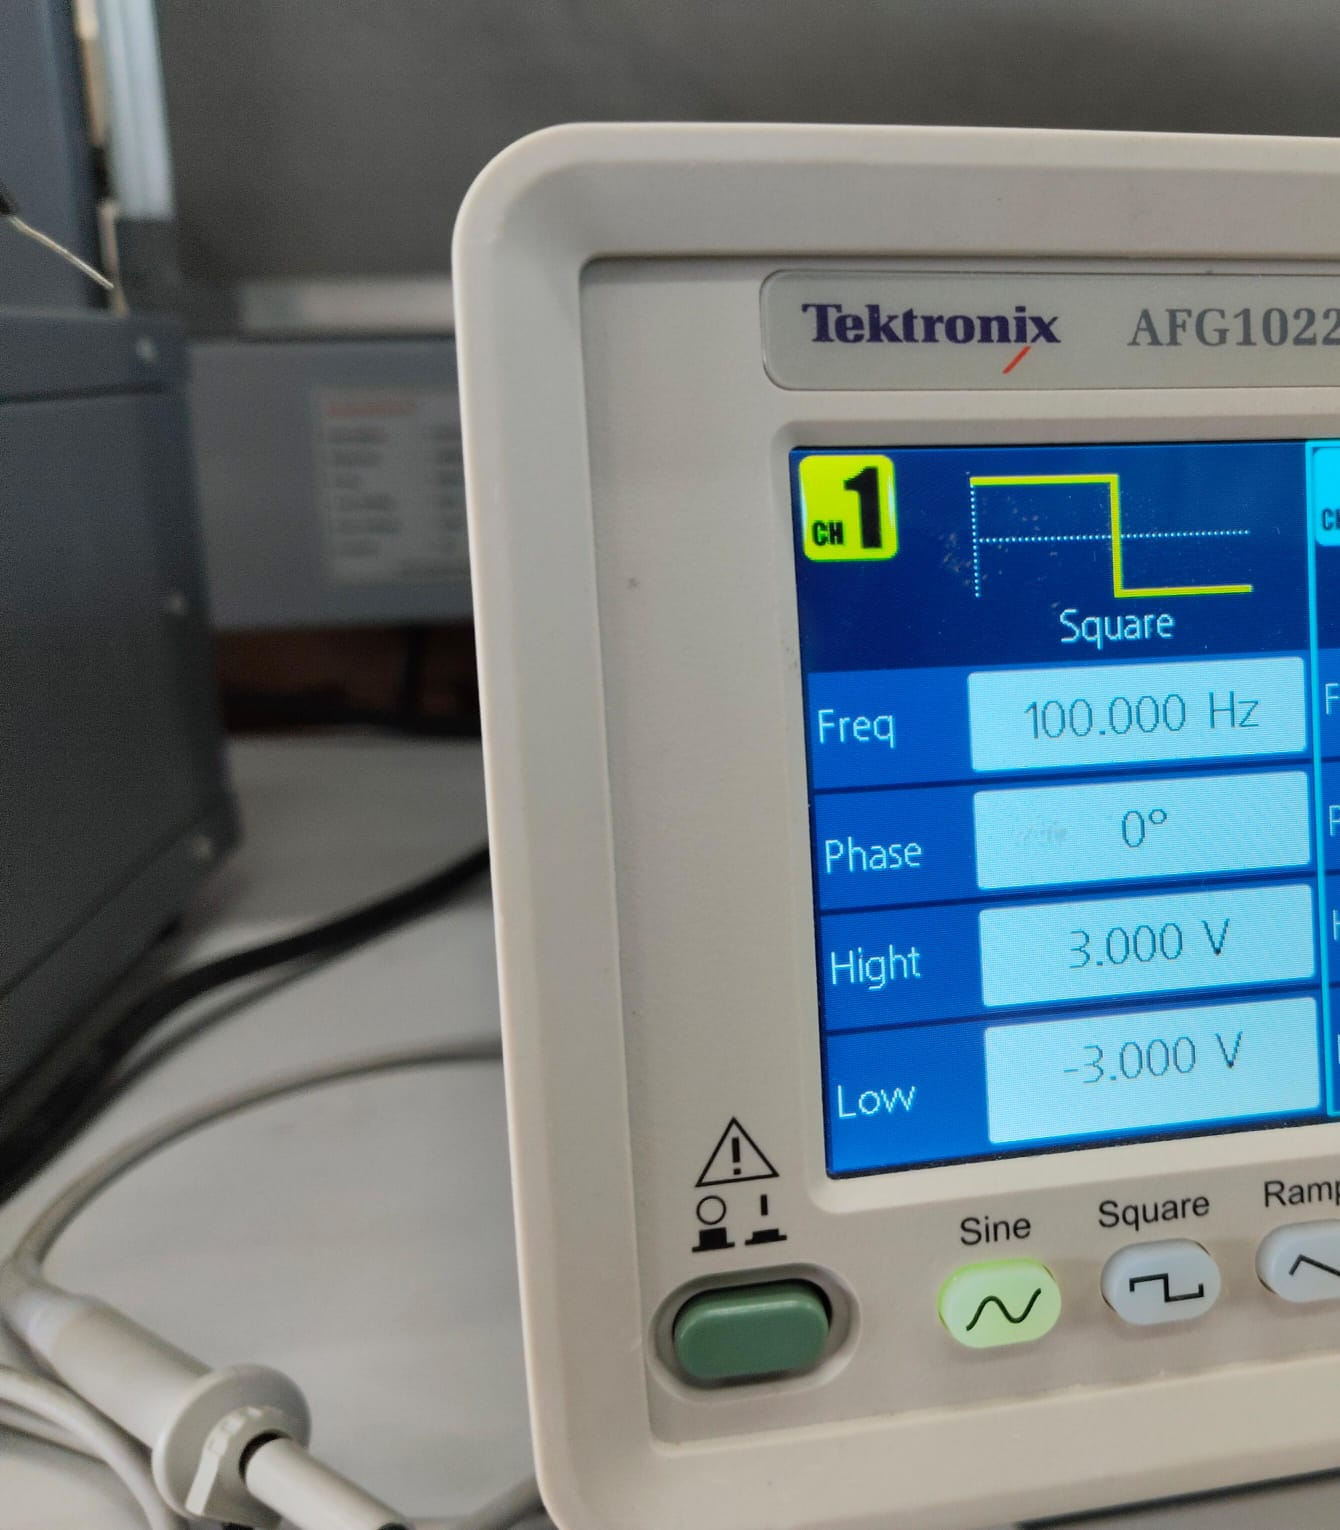
\includegraphics[width=0.4\textwidth]{figs/integrator2.png}
    \caption{Input for Halfwave Rectifier}
\end{figure}
\begin{figure}[H]
    \centering
    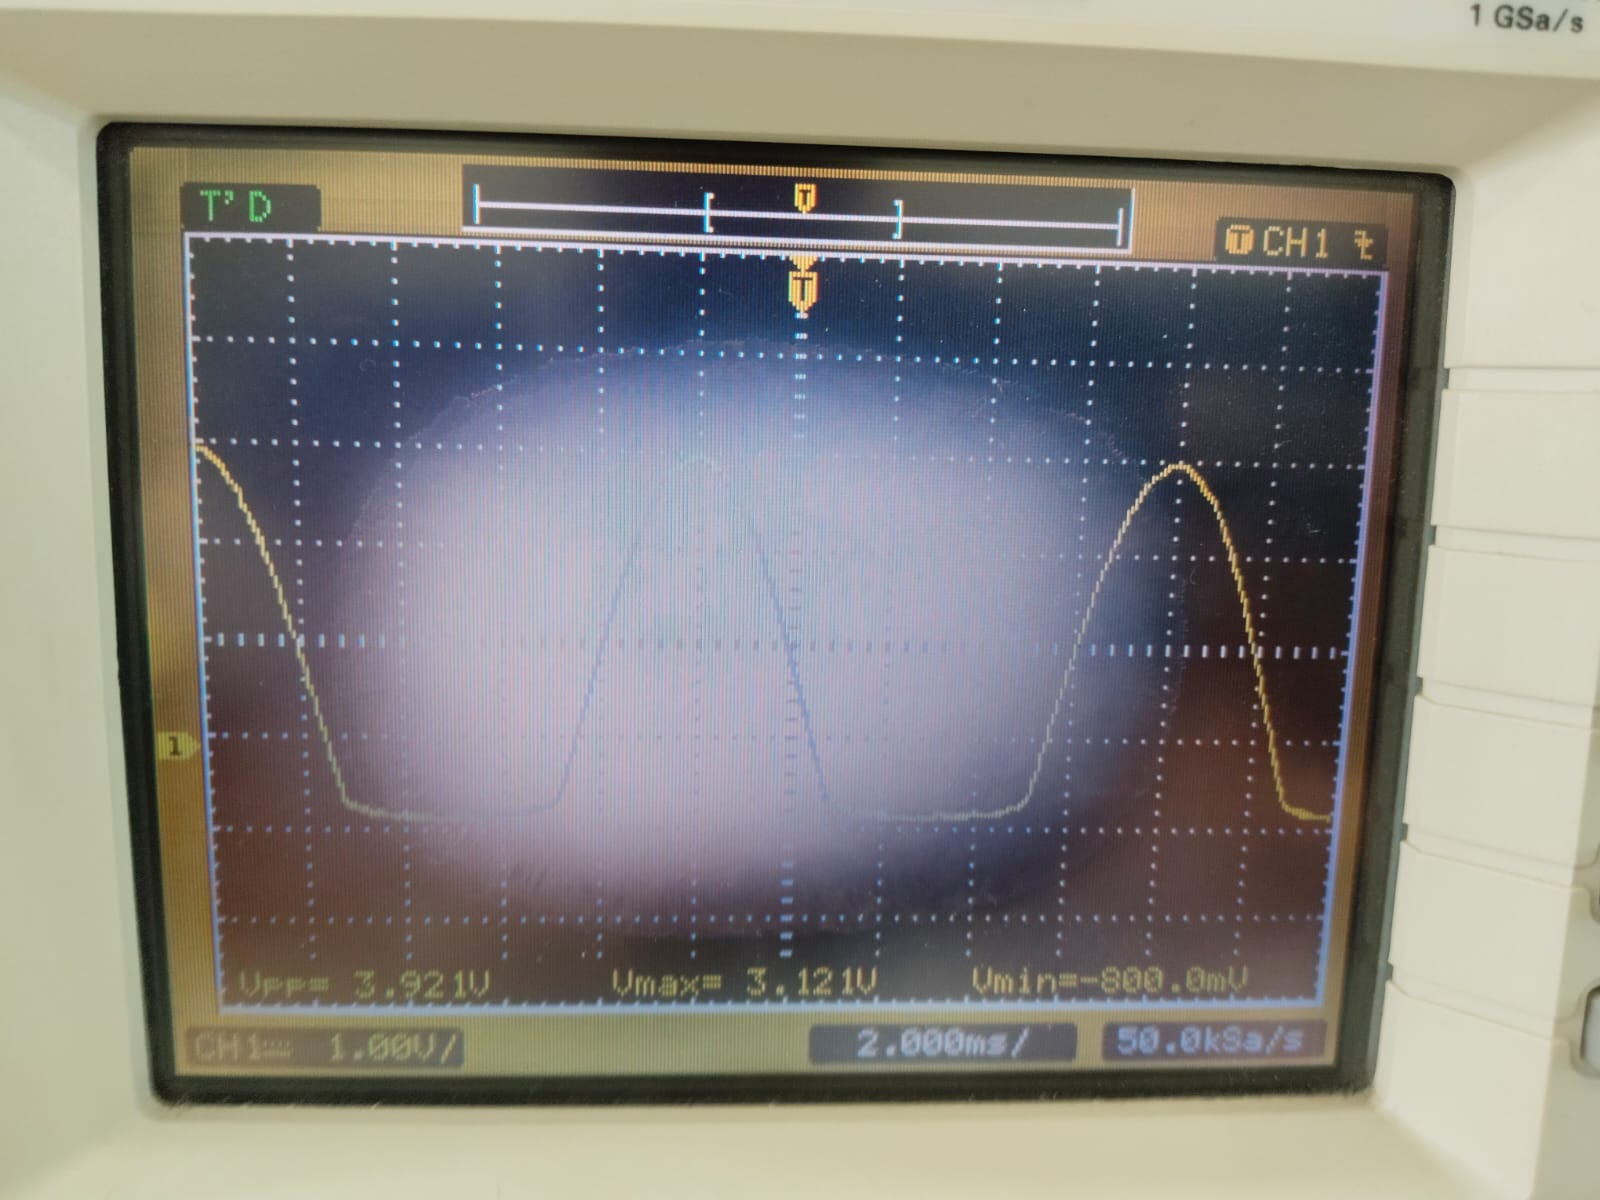
\includegraphics[width=0.5\textwidth]{figs/halfwavevalue.png}
    \caption{Observed Halfwave Precision Rectification}
\end{figure}
\begin{figure}[H]
    \centering
    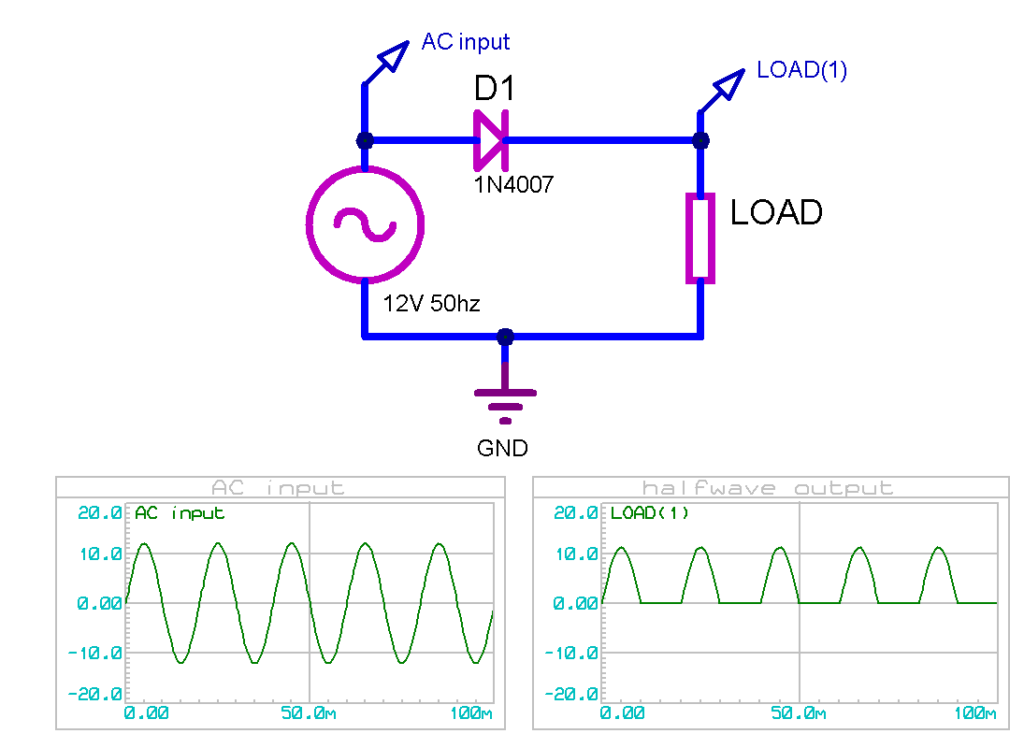
\includegraphics[width=0.7\textwidth]{figs/diode.png}
    \caption{Circuit Diagram for Halfwave Rectification using diode and resistor(values in this are not the one's used for experiment)}
\end{figure}
\begin{figure}[H]
    \centering
    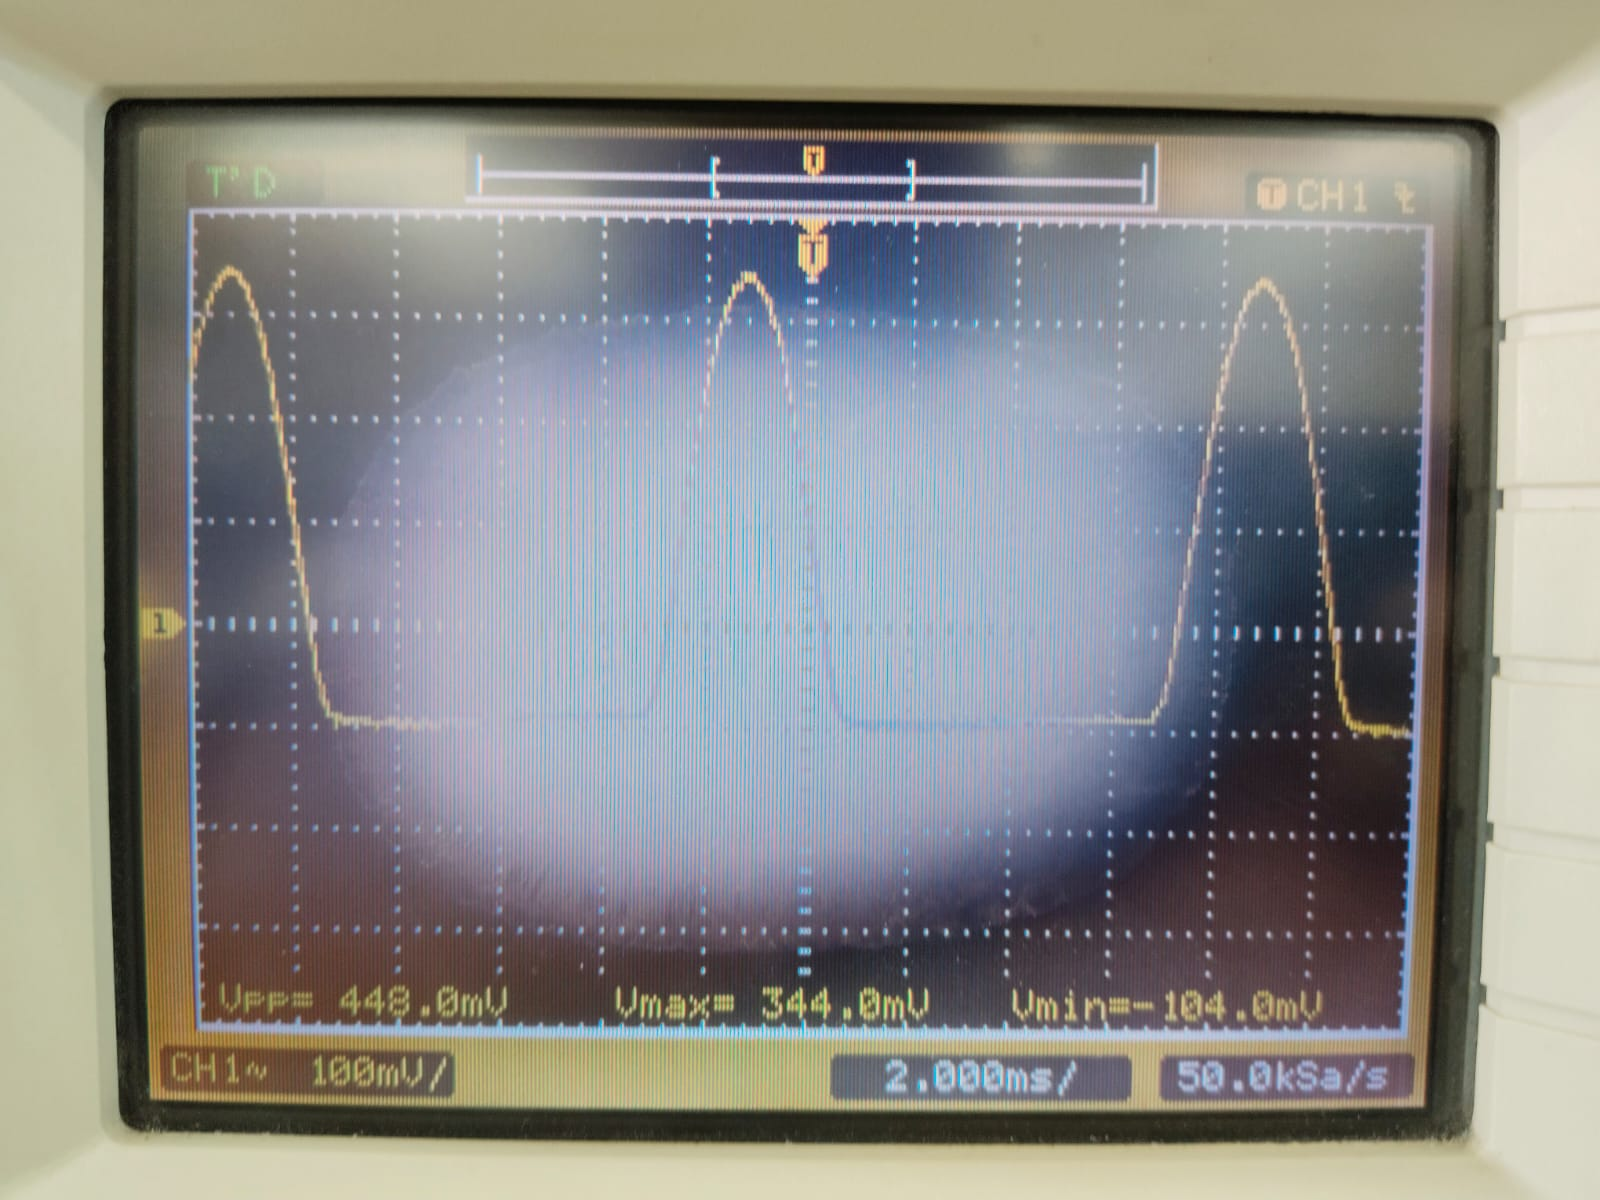
\includegraphics[width=0.5\textwidth]{figs/halfwave_diode.png}
    \caption{Observed Halfwave Rectification without opamp}
\end{figure}
There is the 0.7V threshold voltage of diode hence for given input of 1.2V we should get $1.2V - 0.7V = 0.4V$. The observed value is 0.344V.\\
There is Leakage of current in the diode thats why there is less voltage than theoretical value.

\section{Conclusion}
The experimental results confirm the correct operation of the summing amplifier, op-amp integrator, and precision rectifier. The precision rectifier successfully eliminates the voltage drop of conventional diodes, enabling accurate rectification of small AC signals.

\end{document}
